\documentclass[12pt]{article}
\usepackage[utf8]{inputenc}
\usepackage[T2B]{fontenc}
\usepackage[english,russian]{babel}

\frenchspacing

\usepackage{amsmath}
\usepackage{amssymb}
\usepackage{hyperref}
\usepackage{longtable}
\usepackage[table]{xcolor}
\usepackage{array}
\usepackage{color}
\usepackage{xcolor}
\usepackage{fullpage}
\usepackage{multicol,multirow}
\usepackage{tabularx}
\usepackage{ulem}
\usepackage{listings}
\usepackage{graphicx}
\usepackage{pdfpages}
\usepackage[utf8]{inputenc}
\usepackage[russian]{babel}

\hypersetup{
    colorlinks=true,
    linkcolor=blue,
    filecolor=magenta,
    urlcolor=cyan,
}

\newcommand{\MYhref}[3][blue]{\href{#2}{\color{#1}{#3}}}%

\usepackage{listings}
\usepackage{alltt}
\usepackage{csquotes}
\DeclareQuoteStyle{russian}
	{\guillemotleft}{\guillemotright}[0.025em]
	{\quotedblbase}{\textquotedblleft}
\ExecuteQuoteOptions{style=russian}

\usepackage{graphicx}

\usepackage{listings}
\lstset{tabsize=2,
	breaklines,
	columns=fullflexible,
	flexiblecolumns,
	numbers=left,
	numberstyle={\footnotesize},
	extendedchars,
	inputencoding=utf8}

\usepackage{longtable}

\def\@xobeysp{ }
\def\verbatim@processline{\hspace{1.2cm}\raggedright\the\verbatim@line\par}

\oddsidemargin=-0.4mm
\textwidth=160mm
\topmargin=4.6mm
\textheight=210mm

\parindent=0pt
\parskip=3pt

\definecolor{lightgray}{gray}{0.9}


\renewcommand{\thesubsection}{\arabic{subsection}}

\lstdefinestyle{customc}{
  belowcaptionskip=1\baselineskip,
  breaklines=true,
  frame=L,
  xleftmargin=\parindent,
  language=C,
  showstringspaces=false,
  basicstyle=\footnotesize\ttfamily,
  keywordstyle=\bfseries\color{green!40!black},
  commentstyle=\itshape\color{gray},
  identifierstyle=\color{black},
  stringstyle=\color{blue},
}

\lstdefinestyle{customasm}{
  belowcaptionskip=1\baselineskip,
  frame=L,
  xleftmargin=\parindent,
  language=[x86masm]Assembler,
  basicstyle=\footnotesize\ttfamily,
  commentstyle=\itshape\color{purple!40!black},
}

\lstset{escapechar=@,style=customc}

% Отступы
\usepackage{geometry}
\geometry{
a4paper,
right=10mm,
left=10mm,
top=20mm,
bottom=20mm,
}

% https://tex.stackexchange.com/questions/55698/text-under-a-line
\newcommand\tline[2]{$\underset{\text{#1}}{\text{\underline{\hspace{#2}}}}$}

% Заголовок курсовой работы
% Единственный аргумент --- ее тема

\newcommand{\CWPHeader}[1]{\addtocounter{section}{-1}\section{#1}}

\newcommand{\CWHeader}[1]{\section*{#1}}

\newcommand{\CWProblem}[1]{\par\textbf{Задача: }#1}
\begin{document}
\begin{titlepage}
\begin{center}
\bfseries

{\Large Министерство науки и высшего образования}

\vspace{12pt}

{\Large Московский авиационный институт \\ (национальный исследовательский университет)}

\vspace{48pt}

\large Институт компьютерных наук и прикладной математики

\vspace{36pt}

\large Кафедра вычислительной математики и программирования

\vspace{72pt}

Журнал по ознакомительной практике \\
% (индивидуальный план)

\end{center}

\vspace{180pt}

\begin{flushleft}
\hspace{350pt} Студент: Амурский В. А. 
\vspace{5pt}
\hspace{350pt} Группа: М8О-101Б-21 
\vspace{5pt}
\hspace{350pt} Оценка: 
\vspace{5pt}
\hspace{350pt} Дата: 
\vspace{5pt}
\hspace{350pt} Подпись:
\end{flushleft}

\vspace*{\fill}

\begin{center}
\bfseries
Москва, \the\year
\end{center}
\end{titlepage}

\begin{center}
\bfseries{\large ИНСТРУКЦИЯ }

\vspace{12pt}

\bfseries{о заполнении журнала по производственной практике}
\end{center}

\begin{multicols}{2}
{\small
Журнал по производственной практике студентов имеет единую форму для всех видов практик.

Задание в журнал вписывается руководителем практики от института в первые три-пять дней пребывания студентов на практике в соответствии с тематикой, утверждённой на кафедре до начала практики. Журнал по производственной практике является основным документом для текущего и итогового контроля выполнения заданий, требований инструкции и программы практики.

Табель прохождения практики, задание, а также технический отчёт выполняются каждым студентом самостоятельно.

Журнал заполняется студентом непрерывно в процессе прохождения всей практики и регулярно представляется для просмотра руководителям практики. Все их замечания подлежат немедленному выполнению.

В разделе «Табель прохождения практики» ежедневно должно быть указано, на каких рабочих местах и в качестве кого работал студент. Эти записи проверяются и заверяются цеховыми руководителями практики, в том числе мастерами и бригадирами. График прохождения практики заполняется в соответствии с графиком распределения студентов по рабочим местам практики, утверждённым руководителем предприятия.
В разделе «Рационализаторские предложения» должно быть приведено содержание поданных в цехе рационализаторских предложений со всеми необходимыми расчётами и эскизами. Рационализаторские предложения подаются индивидуально и коллективно.

Выполнение студентом задания по общественно-политической практике заносятся в раздел «Общественно-политическая практика». Выполнение работы по оказанию практической помощи предприятию (участие в выполнении спецзаданий, работа сверхурочно и т.п.) заносятся в раздел журнала «Работа в помощь предприятию» с последующим письменным подтверждением записанной работы соответствующими цеховыми руководителями.
Раздел «Технический отчёт по практике» должен быть заполнен особо тщательно. Записи необходимо делать чернилами в сжатой, но вместе с тем чёткой и ясной форме и технически грамотно. Студент обязан ежедневно подробно излагать содержание работы, выполняемой за каждый день. Содержание этого раздела должно отвечать тем конкретным требованиям, которые предъявляются к техническому отчёту заданием и программой практики. Технический отчёт должен показать умение студента критически оценивать работу данного производственного участка и отразить, в какой степени студент способен применить теоретические знания для решения конкретных производственных задач.

Иллюстративный и другие материалы, использованные студентом в других разделах журнала, в техническом отчёте не должны повторяться, следует ограничиваться лишь ссылкой на него. Участие студентов в производственно-технической конференции, выступление с докладами, рационализаторские предложения и т.п. должны заноситься на свободные страницы журнала.

{\bfseries Примечание.} Синьки, кальки и другие дополнения к журналу могут быть сделаны только с разрешения администрации предприятия и должны подшиваться в конце журнала.

Руководители практики от института обязаны следить за тем, чтобы каждый цеховой руководитель практики перед уходом студентов из данного цеха в другой цех вписывал в журнал студента отзывы об их работе в цехе.

Текущий контроль работы студентов осуществляется руководители практики от института и цеховыми руководителями практики заводов. Все замечания студентам руководители делают в письменном виде на страницах журнала, ставя при этом свою подпись и дату проверки.

Результаты защиты технического отчёта заносятся в протокол и одновременно заносятся в ведомость и зачётную книжку студента.

{\bfseries Примечание.} Нумерация чистых страниц журнала проставляется каждым студентом в своём журнале до начала практики.}
\end{multicols}

\begin{center}
С инструкцией о заполнении журнала ознакомлены:
\end{center}

\enquote{\hspace{0.5cm}} \tline{(дата)}{1.5in} 2022\,г.\hfill Студент Амурский В. А. \tline{(подпись)}{1in}

\pagebreak
\begin{center}
\bfseries{\large ЗАДАНИЕ}
\end{center}

Принять участие в тренировках и соревнованиях по олимпиадному программированию для студентов первого курса в 2021/2022 учебном году: посетить и проработать установочные лекции, решать и дорешивать конкурсные задания, принять участие в разборе. Объём практики 154 часов.

\vspace*{\fill}
Руководитель практики от института:

\vspace{5pt}
\enquote{\hspace{0.5cm}} \tline{(дата)}{1.5in} 2022\,г.\hfill \tline{(подпись)}{1in}
\pagebreak

\begin{center}
\bfseries{\large ТАБЕЛЬ ПРОХОЖДЕНИЯ ПРАКТИКИ}
\end{center}

\resizebox{\columnwidth}{!}{
\begin{tabular}{|c|c|c|c|c|c|c|c|}
\hline
\textbf{№} & \textbf{Дата} & \textbf{Название} & \textbf{Время} & \textbf{Место} & \textbf{Решено} & \textbf{Дорешано} & \textbf{Подпись} \\
& & \textbf{контеста} & \textbf{проведения} & \textbf{проведения} & \textbf{задач} & \textbf{задач} & \\
\hline
1 & 17.09.2021 & Основы C++ [1] & 16:30 - 21:30 & Дистанционно & 0 & 12 & \\
\hline
2 & 19.09.2021 & Stage 2-B: Grand Prix of IMO, Div. 2 & 11:00 - 16:00 & Дистанционно & 2 & 0 & \\
\hline
3 & 24.09.2021 & Основы С++ [2]  & 16:30 - 21:30 & Дистанционно & 0 & 12 & \\
\hline
4 & 26.09.2021 & Stage 3-B: Grand Prix of XiAn, Div. 2 & 11:00 - 16:00 & Дистанционно & 2 & 0 & \\
\hline
5 & 01.10.2021 & Библиотека C++ [3] & 16:30 - 21:30 & Дистанционно & 7 & 5 & \\
\hline
6 & 08.10.2021 & Библиотека C++ [4]  & 16:30 - 21:30 & Дистанционно & 5 & 7 & \\
\hline
7 & 15.10.2021 & Теория чисел [5] & 16:30 - 21:30 & Дистанционно & 3 & 6 & \\
\hline
8 & 22.10.2021 & Основы ДП [6] & 16:30 - 21:30 & Дистанционно & 6 & 6 & \\
\hline
9 & 29.10.2021 & Арифметика в кольце, & 16:30 - 21:30 & Дистанционно & 2 & 8 & \\
& & комбинаторика, функция Эйлера [7] & & & & & \\
\hline
10 & 05.11.2021 & Префиксные суммы, сортировка событий,  & 16:30 - 21:30 & Дистанционно & 4 & 8 & \\
& & метод двух указателей [8] & & & & & \\
\hline
11 & 12.11.2021 & Двумерное ДП, задача о рюкзаке [9] & 16:30 - 21:30 & Дистанционно & 3 & 2 & \\
\hline
12 & 19.11.2021 & Геометрия, тернарный поиск [10] & 16:30 - 21:30 & Дистанционно & 5 & 1 & \\
\hline
13 & 05.12.2021 & Осенняя олимпиада первого курса & 11:00 - 18:30 & МАИ & 5 & 0 & \\
\hline
14 & 19.12.2021 & ICPC. 1/4 финала & 11:00 - 16:00 & Дистанционно & 3 & 0 & \\
\hline
15 & 11.02.2022 & Основы теории графов [11]  & 16:30 - 21:30 & Дистанционно & 3 & 5 & \\
\hline
16 & 18.02.2022 & Кратчайшие пути во взвешенных графах [12]  & 16:30 - 21:30 & Дистанционно & 6 & 2 & \\
\hline
17 & 20.02.2022 & Stage 10-B: Grand Prix of Kyoto, Div 2  & 11:00 - 16:00 & Дистанционно & 2 & 0 & \\
\hline
18 & 25.02.2022 & СНМ, минимальное остовное дерево [13]  & 16:30 - 21:30 & Дистанционно & 3 & 2 & \\
\hline
19 & 04.03.2022 & Деревья, наименьший общий предок [14]  & 16:30 - 21:30 & Дистанционно & 2 & 0 & \\
\hline
20 & 11.03.2022 & Паросочетания в двудольном графе,  & 16:30 - 21:30 & Дистанционно & 1 & 0 & \\
& & потоки в транспортной сети [15]  & & & & & \\
\hline
21 & 18.03.2022 & Строки, Z-функция, хеши,   & 11:00 - 16:00 & Дистанционно & 5 & 0 & \\
& & префиксное дерево [16]   & & & & & \\
\hline
22 & 25.03.2022 & ДП по подмножествам, ДП по профилю [17]  & 16:30 - 21:30 & Дистанционно & 3 & 0 & \\
\hline
23 & 01.04.2022 & Теория игр, функция Шпрага-Гранди [18]   & 16:30 - 21:30 & Дистанционно & 1 & 0 & \\
\hline
24 & 08.04.2022 & Дерево отрезков [19]   & 16:30 - 21:30 & Дистанционно & 5 & 0 & \\
\hline
25 & 15.04.2022 & Дерево отрезков c & 16:30 - 21:30 & Дистанционно & 2 & 0 & \\
& & отложенными обновлениями [20]  & & & & & \\
\hline
26 & 22.04.2022 & Декартово дерево [21]   & 16:30 - 21:30 & Дистанционно & 5 & 0 & \\
\hline
27 & 24.04.2022 & Rucode & 10:00 - 15:00 & Дистанционно & 1 & 0 & \\
\hline
28 & 01.05.2022 & Grand Prix of BSUIR, Div 2 & 11:00 - 16:00 & Дистанционно & 1 & 0 & \\
\hline
29 & 15.05.2022 & Весенняя олимпиада первого курса     & 16:30 - 21:30 & МАИ & 2 & 0 & \\
\hline
30 & 12.07.2022 & Оформление журнала. & 9:00 - 18:00 & МАИ & & & \\
& & Защита практики & & & & & \\
\hline
& & Итого часов & 154 & & & & \\
\hline
\end{tabular}
}
\pagebreak

\begin{center}
\bfseries{\large Отзывы цеховых руководителей практики}
\end{center}

Принято участие в $29$ контестах, прослушаны установочные лекции и разборы задач, дорешаны задачи контестов, оформлен журнал практики. Задание практики выполнено.

\vspace{15pt}

\hfill Тренер Инютин М. А. \tline{(подпись)}{1in}

\vspace{200pt}

\begin{center}
\bfseries{\large Работа в помощь предприятию}
\end{center}

Встречи с представителями ИТ-компаний, сотрудничающих с МАИ.

\pagebreak

\begin{center}
\bfseries{\large ПРОТОКОЛ }

\vspace{12pt}

\bfseries{ЗАЩИТЫ ТЕХНИЧЕСКОГО ОТЧЁТА}
\end{center}
\noindent
по {\itshape ознакомительной практике}

\vspace{8pt}
\noindent
студентом:
\noindent
Амурским Василием Андреевичем

\begin{longtable}{p{7cm}|p{11cm}}
    \hline
    {\bfseries Слушали:} & {\bfseries Постановили:}  \\
    Отчёт практиканта & Считать практику выполненной \\
    & и защищённой на \\
    \rule{0pt}{450pt} & Общая оценка: \underline{\hspace{2in}}\\
    \rule{0pt}{15pt} & \\
    \hline
\end{longtable}

\vfill

\noindent\begin{tabular}{@{}l l l}
Председатель: & Зайцев В. Е. & \underline{\hspace{2in}} \\
Члены: & Сорокин С. А. & \underline{\hspace{2in}} \\
& Инютин М. А. & \underline{\hspace{2in}}
\end{tabular}
\vspace{12pt}

\noindent
Дата: 12 июля \the\year\,г.\hspace{50pt}\textit
\pagebreak
\begin{center}
\bfseries{\large ТЕХНИЧЕСКИЙ ОТЧЁТ ПО ПРАКТИКЕ}
\end{center}

\subsection*{Основы C++ [1]}
\begin{center}
\includegraphics[width=\textwidth]{1A.png}
\end{center}
\subsubsection*{Идея решения}
Идея проста: cчитать два числа, сложить их и вывести. Асимптотика $O(1)$

\subsubsection*{Исходный код}
\begin{lstlisting}
#include <iostream>
#include <string>
#include <unordered_map>
#include <unordered_set>
#include <algorithm>
#include <vector>
#include <cmath>
using namespace std;
typedef long long ll;

int main()
{
	ios_base::sync_with_stdio(false);
	cin.tie(0);
	cout.tie(0);
	ll a, b;
	cin >> a >> b;
	cout << a + b;
	return 0;
}
\end{lstlisting}
\subsubsection*{Фрагмент турнирной таблицы контеста}
\begin{center}
\includegraphics[width=\textwidth]{state1.png}\newline\noindent
\end{center}

\subsubsection*{Выводы}
Задача дорешана. Проблем не возникло, мог решить на конетсте, если бы его не проспал.
\subsection*{Основы C++ [2]}
\begin{center}
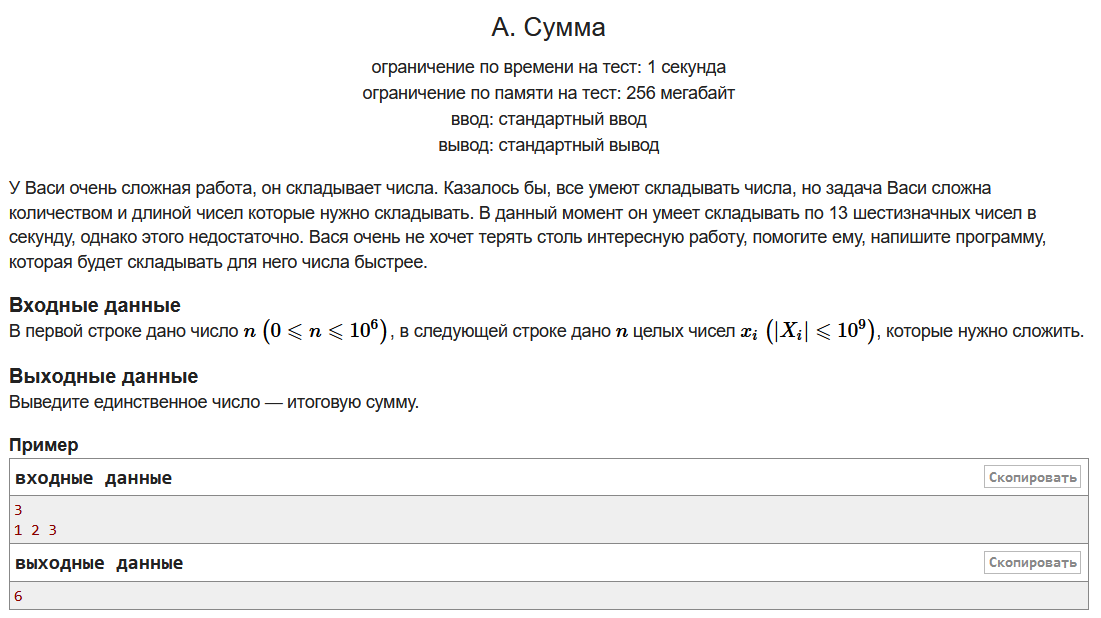
\includegraphics[width=\textwidth]{2A.png}
\end{center}
\subsubsection*{Идея решения}
Сначала заведем массив чисел и введем его через консоль с помощью цикла. Потом так же с помощью цикла просуммируем все числа в массиве и выведем ответ. Асимптотика $O(n)$, где $n$ - кол-во элементов. 
\subsubsection*{Исходный код}
\begin{lstlisting}
#include <iostream>
#include <string>
#include <unordered_map>
#include <unordered_set>
#include <algorithm>
#include <vector>
#include <cmath>
#include <iomanip>
using namespace std;
typedef long long ll;
int main()
{
	ios_base::sync_with_stdio(false);
	cin.tie(0);
	cout.tie(0);
	int n;
	cin >> n;
	ll ans = 0;
	for (int i = 0; i < n; i++) {
		ll x;
		cin >> x;
		ans += x;
	}
	cout << ans;
	return 0;
}
\end{lstlisting}
\subsubsection*{Фрагмент турнирной таблицы контеста}
\begin{center}
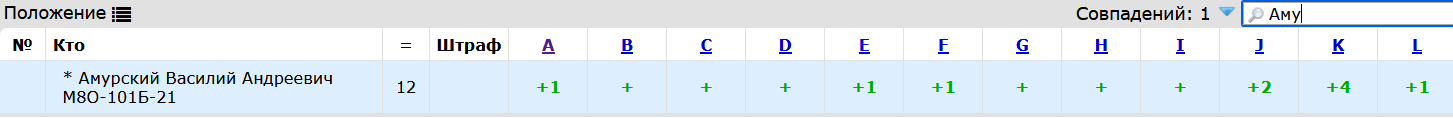
\includegraphics[width=\textwidth]{state2.png}\newline\noindent
\end{center}

\subsubsection*{Выводы}
Задача дорешана. Основные события отладки: неправильный ответ на претесте 1, забыл считать кол-во элементов в массиве.
\subsection*{Библиотека C++ [4]}
\begin{center}
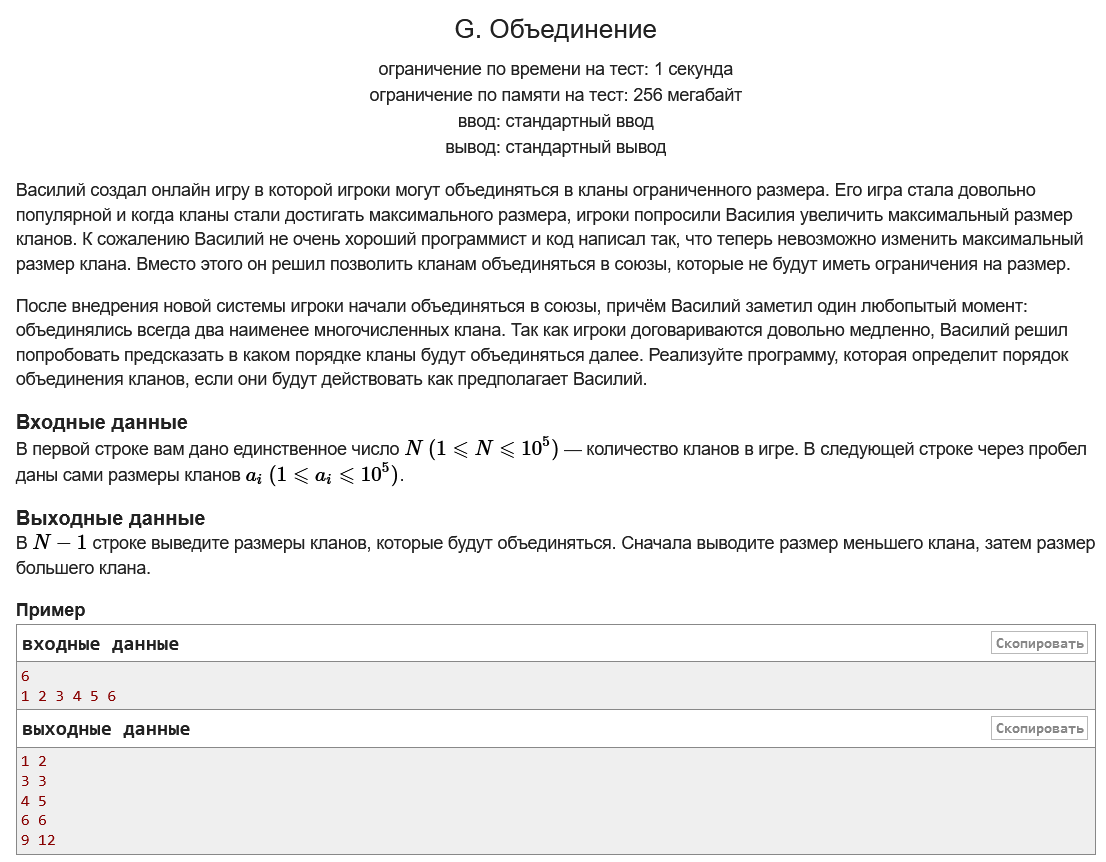
\includegraphics[width=\textwidth]{6G.png}
\end{center}
\subsubsection*{Идея решения}
Будем имитировать численность каждого клана в отсортированном состоянии благодаря типу multiset. Далее заведем цикл с $n-1$ итераций, где будем брать два минимальных элемента, выводить их и класть сумму в multiset. Асимптотика  $O(n\log{}n)$
\subsubsection*{Исходный код}
\begin{lstlisting}
#include <iostream>
#include <string>
#include <unordered_map>
#include <unordered_set>
#include <map>
#include <set>
#include <algorithm>
#include <vector>
#include <cmath>
#include <iomanip>
using namespace std;
typedef long long ll;


int main()
{
    ios_base::sync_with_stdio(false);
    cin.tie(0);
    cout.tie(0);
    ll n;
    cin >> n;
    multiset<ll> a;
    for (int i = 0; i < n; i++) {
        ll x;
        cin >> x;
        a.insert(x);
    }
    for (int i = 0; i < n - 1; i++) {
        ll x1, x2;
        x1 = *a.begin();
        a.erase(a.begin());
        x2 = *a.begin();
        a.erase(a.begin());
        cout << x1 << ' ' << x2 << endl;
        a.insert(x1 + x2);
    }
    return 0;
}
\end{lstlisting}
\subsubsection*{Фрагмент турнирной таблицы контеста}
\begin{center}
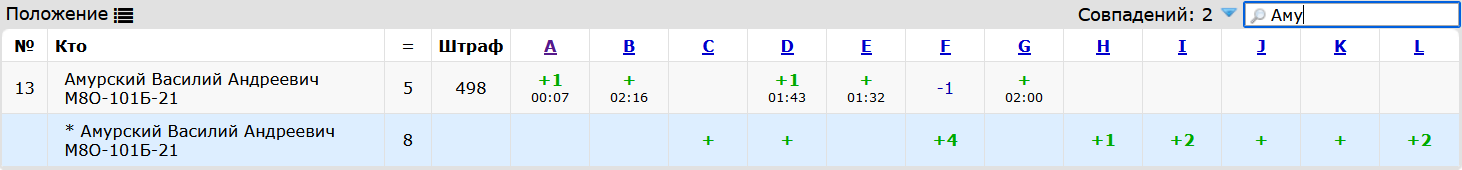
\includegraphics[width=\textwidth]{state6.png}\newline\noindent
\end{center}

\subsubsection*{Выводы}
Задача решена, проблем не возникло.
\subsection*{Арифметика в кольце, комбинаторика, функция Эйлера [7] }
\begin{center}
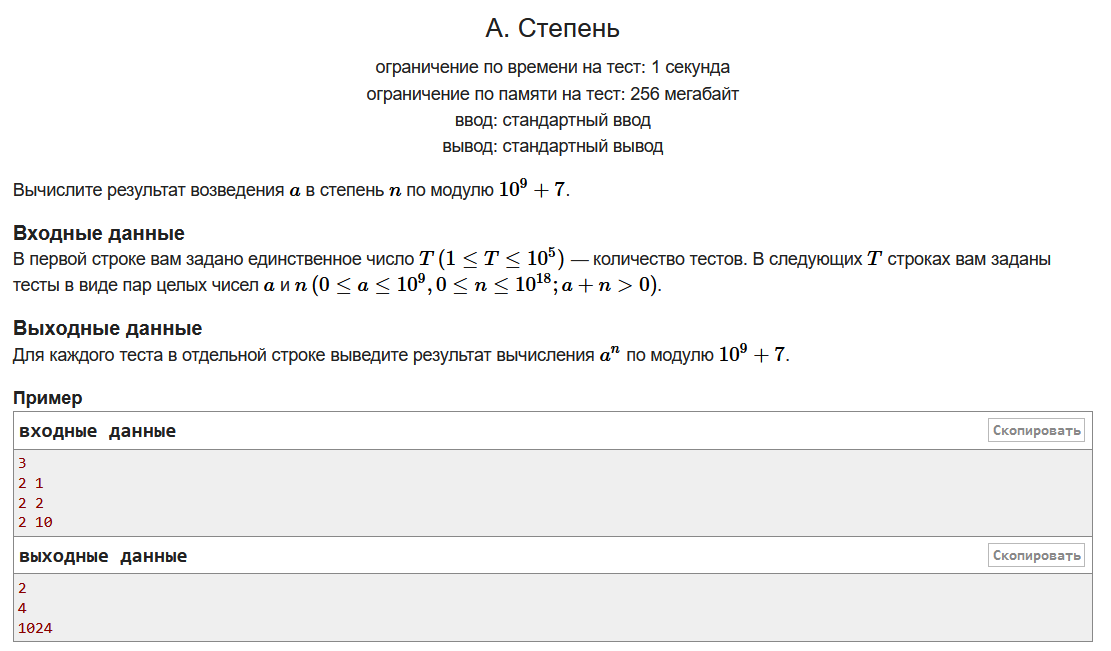
\includegraphics[width=\textwidth]{9A.png}
\end{center}
\subsubsection*{Идея решения}
Реализуем логарифмическое возведение в степень: от степени n мы переходим, если она чётна, к $n / 2$, а иначе — к $n-1$. Понятно, что всего будет не более $2 \log n$ переходов, прежде чем мы придём к $n = 0$. К тому же, после каждого перемножения будем брать остаток по $m=10^9+7$.
\subsubsection*{Исходный код}
\begin{lstlisting}
#include <iostream>
#include <string>
#include <unordered_map>
#include <unordered_set>
#include <map>
#include <set>
#include <algorithm>
#include <vector>
#include <cmath>
#include <numeric>
#include <iomanip>
#include <stack>
#include <fstream>
using namespace std;
typedef long long ll;
ll mod = 1000000007;
int main()
{
    ios_base::sync_with_stdio(false);
    cin.tie(0);
    cout.tie(0);
    ll t;
    cin >> t;
    for (int _ = 0; _ < t; _++) {
        ll res = 1;
        ll a, n;
        cin >> a >> n;
        while (n > 0) {
            if (n % 2 == 1) {
                res = (res * a) % mod;
            }
            a = (a * a) % mod;
            n /= 2;
        }
        cout << res << endl;
    }
    return 0;
}
\end{lstlisting}
\subsubsection*{Фрагмент турнирной таблицы контеста}
\begin{center}
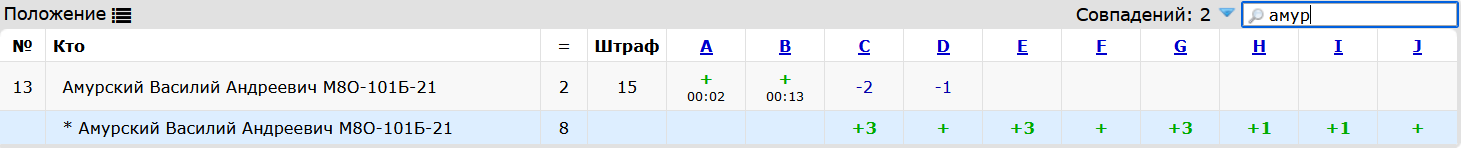
\includegraphics[width=\textwidth]{state9.png}\newline\noindent
\end{center}

\subsubsection*{Выводы}
Задача решена, проблем не возникло.
\end{document}
